\section{Coherent fields and precessing nuclear spins}\label{sec:14.6}

An axion-like field of mass \SI{1}{neV} oscillates at \SI{241.8}{kHz}, and its phase wanders on a time of about a second. A $^{207}$Pb nucleus in a field of \SI{26.8}{mT} precesses at the same frequency. Over a record shorter than a second the field acts on the nuclear spins as one classical wave with a fixed amplitude and phase, the spins tip together, and their transverse magnetization grows in proportion to the time until the spin coherence time $T_2$ caps it, after \SI{17}{ms} in the ferroelectric PMN-PT. The amplitude of the field then changes only on the scale of a second. Whether the golden-rule rate describes such a record depends on the shorter of the two times, and how the sensitivity of a search grows with the length of the record depends on the statistics of the random amplitude.

\subsection{The coherent classical-field regime}\label{sec:14.6-regime}

A light boson of mass $m_\phi$ has about $\rho_\chi/(m_\phi^4v_0^3)$ quanta in a volume $(1/m_\phi v_0)^3$, $4.6\times10^{39}$ at \SI{1}{neV}, and below a few eV it is a classical field (\cref{sec:8.2-absorption}). It is a sum of modes with random phases, one for each velocity in the halo, and by the central limit theorem a Gaussian random field~\cite[Eqs.~(3)--(10)]{foster2018revealing}. A Gaussian field with zero mean is fixed by its two-point function. For a free nonrelativistic field with the velocity distribution $f_\chi(\vect{v})$ of \cref{sec:1.2}, each mode oscillates at $\omega_{\vect{v}} = m_\phi(1 + v^2/2)$, and the average over the random phases is
\begin{equation*}
  \langle\phi(\vect{x},t)\,\phi(\vect{x}',t')\rangle = \frac{\rho_\chi}{m_\phi^2}\int\dd^3v\,f_\chi(\vect{v})\cos\bigl[\omega_{\vect{v}}(t - t') - m_\phi\vect{v}\cdot(\vect{x} - \vect{x}')\bigr] ,
\end{equation*}
normalized so that $\langle\phi^2\rangle = \rho_\chi/m_\phi^2$, the mean square of a wave $\phi_0\cos(m_\phi t)$ with $\tfrac12m_\phi^2\phi_0^2 = \rho_\chi$. With the transforms of \cref{app:A.3} in space and time, the power spectrum of the field is
\begin{equation}
  \mathcal{S}_\phi(\vect{k},\omega) = \frac{\pi\rho_\chi}{m_\phi^2}\,(2\pi)^3\!\int\dd^3v\,f_\chi(\vect{v})\Bigl[\delta^3(\vect{k} + m_\phi\vect{v})\,\delta(\omega - \omega_{\vect{v}}) + \delta^3(\vect{k} - m_\phi\vect{v})\,\delta(\omega + \omega_{\vect{v}})\Bigr] .
  \label{eq:14.6-Sphi}
\end{equation}
The positive-frequency weight sits at $\vect{k} = -m_\phi\vect{v}$ in the sign convention of \cref{eq:A.3-space,eq:A.3-time}, while the target receives the momentum $\vect{p}_\phi = m_\phi\vect{v}$, as in \cref{eq:8.2-abs}; the sign matters only for targets whose response is odd in $\vect{q}$ (\cref{sec:14.5}). Integrated over $\vect{k}$, the positive-frequency part is $(\pi\rho_\chi/m_\phi^2)F_\phi(\omega)$, with
\begin{equation}
  F_\phi(\omega)\,\dd\omega = F_\chi(v)\,\dd v, \qquad \omega - m_\phi = \tfrac12m_\phi v^2 ,
  \label{eq:14.6-Fphi}
\end{equation}
the energy distribution of the field of \cref{sec:11.8}, normalized to one and inherited from the laboratory speed distribution $F_\chi$ of \cref{sec:1.2}. The line is one-sided: it starts at $m_\phi$ and ends at $m_\phi(1 + v_{\mathrm{max}}^2/2)$, $3.5\times10^{-6}$ above it.

The width of the line sets the coherence time. We define it, as \cref{sec:8.2-absorption} estimated it, by
\begin{equation}
  t_{\mathrm{coh}} = \frac{1}{m_\phi v_0^2} = \SI{1.04}{s}\times\frac{\SI{1}{neV}}{m_\phi} ,
  \label{eq:14.6-tcoh}
\end{equation}
with $v_0 = \SI{238}{km/s}$. For the halo of \cref{sec:1.2} seen from the Earth, $F_\phi$ peaks at $0.58/t_{\mathrm{coh}}$ above $m_\phi$, its equivalent width $\Delta\omega_{\mathrm{eq}} = [\int\dd\omega\,F_\phi^2]^{-1}$ is $2.67/t_{\mathrm{coh}}$, and the correlation of the complex amplitude of the field with itself, $|\int\dd\omega\,F_\phi(\omega)\,\ee^{-\ii\omega t}|$, falls to one half at $t = 1.47\,t_{\mathrm{coh}}$. Over the coherence length $1/m_\phi v_0$, \SI{249}{km} at \SI{1}{neV}, the field is uniform, and every laboratory sample sees the same amplitude.

A coupling $\sum_bg^\phi_bO_b$ of the absorption rows of \cref{sec:8.1-absorption} drives the expectation value of any readout operator $O_{\mathrm{rd}}$ through the Kubo formula \cref{eq:4.1-kubo}, with the retarded response $R_{\mathrm{rd},b}(\vect{p}_\phi,t)$. The readout can be the operator that the field couples to, as for the magnetization of the spins below, or another, as for the voltage across a piezoelectric resonator (\cref{sec:11.8}). Either way the signal is linear in the amplitude of the field and in the coupling. Its square averaged over the Gaussian ensemble is quadratic in both and contains $\mathcal{S}_\phi$. The energy that the target absorbs is the case $O_{\mathrm{rd}} = \sum_bg^\phi_bO_b$, and its average reproduces the golden rule, but only after a long enough record. Take the coupling on from $t' = 0$ to $t$. The amplitude of a transition $i \to f$ driven by one mode of frequency $\omega$ contains $\int_0^t\dd t'\,\ee^{\ii(E_f - E_i - \omega)t'}$, whose square is $2\pi t\,\mathcal{K}_t(\omega - E_f + E_i)$ with the Fejér kernel
\begin{equation}
  \mathcal{K}_t(x) = \frac{t}{2\pi}\,\frac{\sin^2(xt/2)}{(xt/2)^2}, \qquad \int\dd x\,\mathcal{K}_t(x) = 1 .
  \label{eq:14.6-fejer}
\end{equation}
The Gaussian average removes the cross terms between modes, as in \cref{app:D.25}, and the mean number of quanta absorbed per unit volume in the record is $t\,(\rho_\chi/m_\phi)$ times the rate \cref{eq:8.2-abs} averaged over the line $F_\phi$, with the $\delta(\omega - E_f + E_i)$ in $S_{ab}$ replaced by $\mathcal{K}_t$. As $t \to \infty$ the kernel becomes the delta function and the mean is the golden-rule rate times $t$. The replacement matters only where both the field line and the target line are narrow compared with $1/t$. Since the kernel acts on their convolution, whose width is at least the larger of the two widths, the golden-rule mean holds for
\begin{equation*}
  t \gg \min\bigl(t_{\mathrm{coh}},\,1/\varGamma_{\mathrm{tg}}\bigr) .
\end{equation*}
Here $\varGamma_{\mathrm{tg}}$ is the width of the target's line: $1/T_2$ for nuclear spins, the full width $\varGamma_{\mathrm{M}}$ of a magnon line (\cref{sec:14.3}), $\gamma_n$ for a resonator mode (\cref{sec:11.8}). For a record shorter than both, the energy absorbed grows as $t^2$. That is the regime of a nuclear spin driven by a field of neV mass over a record shorter than its $T_2$, the coherent regime that \cref{sec:8.2-absorption} named.

The golden-rule mean is not yet what one record measures. A single realization of the field matches the ensemble only when the record spans many coherence times, so that it samples many independent amplitudes. For a detector that counts absorbed quanta, the intensity $|\Phi|^2$ of the complex amplitude $\Phi$ of the field is exponentially distributed within one coherence time, and a record of $N_{\mathrm{coh}}$ independent coherence times gives $\mathrm{Var}\,N = \bar N + \bar N^2/N_{\mathrm{coh}}$, the bunching of chaotic light. The Poisson statistics of \cref{eq:1.5-poisson} hold when $N_{\mathrm{coh}} \gg \bar N$, which counting searches satisfy by a wide margin: the YIG search of \cref{we:14-yig} at \SI{10}{\micro eV} sees 35 events per hour in $3.4\times10^7$ coherence times. A readout of the mean field, such as the magnetization below, is a different matter, since its signal is proportional to the amplitude of the field rather than to its intensity.

\subsection{Bloch equations and nuclear magnetic resonance}\label{sec:14.6-bloch}

A nucleus with spin $\vect{J}^{\mathrm{nuc}}$ and magnetic moment $\mu_{\mathrm{nuc}}$ in a static field $\vect{B}_0 = B_0\hat{\vect{z}}$ has the Zeeman energy $-\omega_{\mathrm{Lar}}J^{\mathrm{nuc}}_z$, with the Larmor frequency $\omega_{\mathrm{Lar}} = \mu_{\mathrm{nuc}}B_0/J_{\mathrm{nuc}}$; for $\mu_{\mathrm{nuc}} > 0$ the lower levels have the spin along the field. A Hamiltonian $-\vect{b}\cdot\vect{J}^{\mathrm{nuc}}$, with $\vect{b}$ a vector of energy, makes the spin precess, $\dd\vect{J}^{\mathrm{nuc}}/\dd t = \vect{J}^{\mathrm{nuc}}\times\vect{b}$; the Zeeman term has $\vect{b} = \omega_{\mathrm{Lar}}\hat{\vect{z}}$. For $^{207}$Pb, with $J_{\mathrm{nuc}} = \frac12$ and $\mu_{\mathrm{nuc}} = 0.5926$ nuclear magnetons, $\omega_{\mathrm{Lar}}/2\pi = \SI{9.03}{MHz}$ per tesla~\cite[Eq.~(S11)]{aybas2021search}.

A sample of $\nd_{\mathrm{nuc}}$ such nuclei per unit volume carries the magnetization $\vect{M}$, equal to $\nd_{\mathrm{nuc}}\mu_{\mathrm{nuc}}/J_{\mathrm{nuc}}$ times $\langle\vect{J}^{\mathrm{nuc}}\rangle$, and a spin $\frac12$ in equilibrium has the polarization $p_{\mathrm{pol}} = 2\langle J^{\mathrm{nuc}}_z\rangle = \tanh(\omega_{\mathrm{Lar}}/2T)$ and $M_0 = \nd_{\mathrm{nuc}}\mu_{\mathrm{nuc}}p_{\mathrm{pol}}$. For $^{207}$Pb at \SI{4.4}{T} and \SI{4.2}{K}, $p_{\mathrm{pol}} = 2.3\times10^{-4}$, and with $\nd_{\mathrm{nuc}} = \SI{3.4e27}{m^{-3}}$ in PMN-PT, a relaxor ferroelectric of lead magnesium niobate and lead titanate, $\mu_0M_0 = \SI{2.9}{nT}$, the equilibrium value of Aybas and collaborators~\cite[Eqs.~(S12), (S13)]{aybas2021search}. Searches therefore polarize the spins in a large field, or optically, and then work at a lower field while the polarization relaxes; the sample is out of equilibrium, with a polarization fixed by its preparation.

The averaged spins obey the same precession, with two relaxation times added phenomenologically by Bloch~\cite{bloch1946nuclear}:
\begin{equation}
  \frac{\dd\vect{M}}{\dd t} = \vect{M}\times\vect{b}(t) - \frac{M_x\hat{\vect{x}} + M_y\hat{\vect{y}}}{T_2} - \frac{M_z - M_0}{T_1}\,\hat{\vect{z}} ,
  \label{eq:14.6-bloch}
\end{equation}
with $\vect{b}(t) = \omega_{\mathrm{Lar}}\hat{\vect{z}} + \vect{b}_\phi(t)$ including any drive. The longitudinal time $T_1$ is set by the exchange of energy with the lattice and reaches hours in insulators at cryogenic temperatures~\cite{budker2014proposal}. The transverse time $T_2$ is set by the loss of phase between spins, mainly through their magnetic dipole interactions, and is of order a millisecond in a solid; pulse sequences that average the dipolar coupling extend it by orders of magnitude. For $^{207}$Pb in PMN-PT, $T_2 = \SI{16.7}{ms}$. Spins at inequivalent sites, or with different chemical shifts, precess at different frequencies, and this inhomogeneous broadening spreads the resonance of the whole sample over a width $\varGamma_{\mathrm{inh}}$, $2\pi\times\SI{78}{kHz}$ in PMN-PT~\cite[Eqs.~(S24), (S25)]{aybas2021search}. In the response formalism, the spins form an absorber with a Lorentzian line. With the transverse decay $\ee^{-t/T_2}$ inserted in \cref{eq:4.1-kubo}, the operator $J^{\mathrm{nuc}}_-$, which raises the Zeeman energy by $\omega_{\mathrm{Lar}}$, has the retarded response
\begin{equation*}
  R_{J_-J_-}(\omega) = \frac{2\langle J^{\mathrm{nuc}}_{z,\mathrm{tot}}\rangle/\Vol}{\omega - \omega_{\mathrm{Lar}} + \ii/T_2} ,
\end{equation*}
from $\langle[J_+, J_-]\rangle = 2\langle J_z\rangle$ for the total spin of the sample. Its imaginary part is negative, an absorber in the sense of \cref{sec:4.2}, only if $\langle J^{\mathrm{nuc}}_z\rangle > 0$, that is, if the lower Zeeman levels are the more populated.

\subsection{The nuclear-spin precession signal}\label{sec:14.6-signal}

Two couplings of an axion-like field reach the nuclear spins. The first is the gradient coupling of \cref{sec:11.6-spins}: each nucleus of isotope $i$ feels $(g_{ai}/m_N)(\nabla\phi)\cdot\vect{J}^{\mathrm{nuc}}$, the nuclear spin row of \cref{eq:8.1-rows} with the coefficient $g^\phi_{s_i,a} = \ii g_{ai}p_{\phi,a}/m_N$. \Cref{sec:11.6-spins} found that this term does not reach the phonons, since its final states sit at the spin splittings; an applied field moves those splittings up to $m_\phi$. For a wave $\phi_0\cos(m_\phi t - \vect{p}_\phi\cdot\vect{x})$ the coupling is $-\vect{b}_\phi\cdot\vect{J}^{\mathrm{nuc}}$ with
\begin{equation*}
  \vect{b}_\phi(t) = -\frac{g_{ai}}{m_N}\,\sqrt{2\rho_\chi}\;\vect{v}\,\sin(m_\phi t) ,
\end{equation*}
at the sample, a pseudo-magnetic field along the velocity of the dark matter. Aybas and collaborators write the same coupling with $g_{aNN} = g_{ai}/m_N$~\cite[Eqs.~(S49)--(S53)]{aybas2021search}. The second coupling is the oscillating electric dipole moment that an axion induces in nucleons, $d_n = g_d\phi$. In a polar crystal the electrons screen the electric field at the nucleus, and what survives, through the Schiff moment (the part of the nuclear electric-dipole distribution that the screening leaves), is an energy shift $\pm\Delta\varepsilon(t)$ of the two levels of a spin $\frac12$ quantized along an effective field $\vect{E}^*$ fixed by the crystal~\cite{budker2014proposal}. That is again a spin coupling, with $\vect{b}_\phi = 2\Delta\varepsilon(t)\hat{\vect{E}}^*$. For $^{207}$Pb in PMN-PT, $\Delta\varepsilon = d_nE^*$ with $E^* = \SI{340}{kV/cm}$, uncertain by about \SI{50}{\percent}~\cite[Eqs.~(S44), (S45)]{aybas2021search}. The scalar couplings of \cref{sec:8.1-absorption} act on orbital coordinates and leave the nuclear spins alone, as for the electron spins of \cref{sec:14.3}.

Only the component of $\vect{b}_\phi$ transverse to $\vect{B}_0$ tips the spins. A linear drive $b_\perp\cos(m_\phi t)\hat{\vect{x}}$ is the sum of two circular components of amplitude $b_\perp/2$, and near resonance only the one that rotates with the precession acts. In the frame that rotates at $m_\phi$, and dropping the counter-rotating component, the spins see a static field of strength
\begin{equation*}
  \Omega_{\mathrm{Rabi}} = \tfrac12 b_\perp ,
\end{equation*}
with the detuning $\delta\omega_{\mathrm{Lar}} = \omega_{\mathrm{Lar}} - m_\phi$. For the gradient coupling $\Omega_{\mathrm{Rabi}} = g_{ai}\sqrt{2\rho_\chi}\,v_\perp/2m_N$, and for the dipole coupling of a spin $\frac12$ with $\vect{E}^*\perp\vect{B}_0$, $\Omega_{\mathrm{Rabi}} = \Delta\varepsilon$, the shift of each level. Write $M_+ = M_x + \ii M_y$. In \cref{eq:14.6-bloch} the precession about $\vect{B}_0$ gives $\dd M_+/\dd t = -\ii\omega_{\mathrm{Lar}}M_+$, and the drive adds $\ii b_\perp\cos(m_\phi t)M_z$. As long as the spins are barely tipped, $M_z = M_0$. For $\tilde M_+ = \ee^{\ii m_\phi t}M_+$, keeping the co-rotating half of the drive,
\begin{equation*}
  \frac{\dd\tilde M_+}{\dd t} = -\Bigl(\ii\delta\omega_{\mathrm{Lar}} + \frac{1}{T_2}\Bigr)\tilde M_+ + \ii\,\Omega_{\mathrm{Rabi}}M_0 ,
\end{equation*}
a linear equation with a constant source. With the spins along the field at $t = 0$, $\tilde M_+(0) = 0$, its solution is the magnetization that a search records.
\begin{keyresult}[Transverse magnetization of a driven nuclear-spin ensemble]
\begin{equation}
  \begin{gathered}
  \tilde M_+(t) = \ii\,\Omega_{\mathrm{Rabi}}M_0\,\frac{1 - \ee^{-(\ii\delta\omega_{\mathrm{Lar}} + 1/T_2)t}}{\ii\delta\omega_{\mathrm{Lar}} + 1/T_2} , \\
  |M_\perp| = \Omega_{\mathrm{Rabi}}M_0\,\frac{2|\sin(\delta\omega_{\mathrm{Lar}}t/2)|}{|\delta\omega_{\mathrm{Lar}}|}\quad(t \ll T_2), \\
  |M_\perp| = \frac{\Omega_{\mathrm{Rabi}}M_0T_2}{(1 + \delta\omega_{\mathrm{Lar}}^2T_2^2)^{1/2}}\quad(t \gg T_2),
  \end{gathered}
  \label{eq:14.6-mperp}
\end{equation}
for a field of fixed amplitude and phase, with $\Omega_{\mathrm{Rabi}}t \ll 1$ and $\Omega_{\mathrm{Rabi}}^2T_1T_2 \ll 1$. The magnetization precesses at $m_\phi$ in the laboratory, about $\vect{B}_0$.
\end{keyresult}
\noindent On resonance the magnetization grows linearly, $|M_\perp| = \Omega_{\mathrm{Rabi}}M_0t$, until $T_2$ caps it at $\Omega_{\mathrm{Rabi}}M_0T_2$. For the whole sample the steady state is $M_\perp = u_{\mathrm{sp}}M_0\Omega_{\mathrm{Rabi}}T_2$~\cite[Eq.~(1)]{aybas2021search}. The spectral factor $u_{\mathrm{sp}}$ averages the Lorentzian of \cref{eq:14.6-mperp} over the inhomogeneous line, $u_{\mathrm{sp}} \simeq \pi/(\varGamma_{\mathrm{inh}}T_2) = 3.8\times10^{-4}$ for $^{207}$Pb in PMN-PT~\cite[Eqs.~(S22)--(S25)]{aybas2021search}: only the spins within about $1/T_2$ of $m_\phi$ respond, a fraction $u_{\mathrm{sp}}$ of the sample. The steady state is also the Kubo response of the magnetization, $\langle J_+\rangle$ driven through $R_{J_-J_-}$ of \cref{sec:14.6-bloch}. The imaginary part of the same response, inserted in \cref{eq:8.2-abs}, is the rate at which the spins absorb quanta.

The drive is the Gaussian field of \cref{eq:14.6-Sphi}, whose complex amplitude in the rotating frame wanders on the scale $t_{\mathrm{coh}}$. Let $\Omega_{\mathrm{rms}}$ be the Rabi frequency of a fixed wave with the mean energy density, $\phi_0 = \sqrt{2\rho_\chi}/m_\phi$. For the gradient coupling, whose direction is random as well, we replace $v_\perp^2$ by its average $\langle v_\perp^2\rangle$; this is an approximation, since $v_\perp^2$ is correlated with the speed and hence with $\omega$, and the exact form weights the line by the mean of $v_\perp^2$ at each speed. The equation for $\tilde M_+$ is linear, so each mode of the field contributes its own solution of the form \cref{eq:14.6-mperp}, at its own detuning, and the Gaussian average adds their squares:
\begin{equation}
  \bigl\langle|M_\perp(t)|^2\bigr\rangle = \Omega_{\mathrm{rms}}^2M_0^2\int\dd\omega\,F_\phi(\omega)\,\frac{\bigl|1 - \ee^{-[\ii(\omega_{\mathrm{Lar}} - \omega) + 1/T_2]t}\bigr|^2}{(\omega_{\mathrm{Lar}} - \omega)^2 + 1/T_2^2} .
  \label{eq:14.6-ms}
\end{equation}
For $t \ll t_{\mathrm{coh}}$ all modes are in phase over the record, and the magnetization has the form \cref{eq:14.6-mperp} with a random amplitude: $|M_\perp|$ is Rayleigh distributed, and its square is exponential with the mean $\Omega_{\mathrm{rms}}^2M_0^2t^2$ on resonance. For $t_{\mathrm{coh}} \ll t \ll T_2$ the phase of the drive wanders and the magnetization random-walks, $\langle|M_\perp|^2\rangle = 2\pi F_\phi(\omega_{\mathrm{Lar}})\,\Omega_{\mathrm{rms}}^2M_0^2\,t$. For $t \gg T_2$ it saturates, at $\pi F_\phi(\omega_{\mathrm{Lar}})\,\Omega_{\mathrm{rms}}^2M_0^2\,T_2$ if $T_2 \gg t_{\mathrm{coh}}$, the balance between the golden-rule rate of \cref{eq:8.2-abs} and the decay $1/T_2$. If instead $T_2 \ll t_{\mathrm{coh}}$, the spin line is broad compared with the field line, and the fixed-amplitude steady state with a Rayleigh amplitude holds at every time. \Cref{lim:14.6a} shows both cases.
\begin{limitbox}[Transverse magnetization of a driven nuclear-spin ensemble][lim:14.6a]
$|M_\perp| = \Omega_{\mathrm{Rabi}}M_0t$ for $t \ll T_2$ and $\Omega_{\mathrm{Rabi}}M_0T_2$ for $t \gg T_2$, on resonance, for a drive of fixed amplitude~\cites[Eq.~(1)]{budker2014proposal}[Eq.~(1)]{aybas2021search}.
\par\smallskip
{\centering
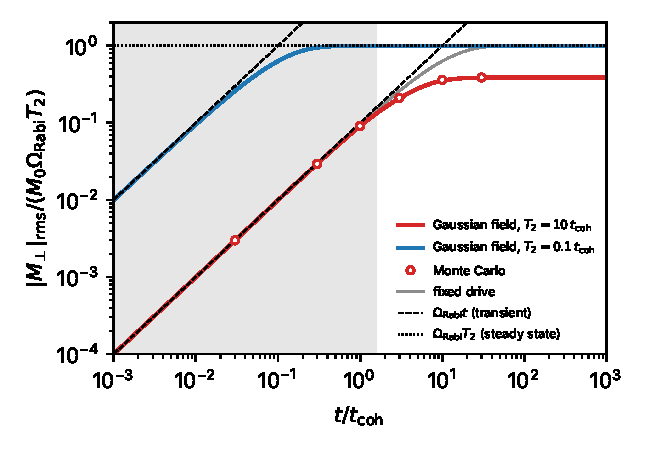
\includegraphics[width=0.92\linewidth]{figures/ch14/limit14_6a.pdf}
\captionof{figure}{Root-mean-square transverse magnetization of a nuclear-spin ensemble driven on resonance by an axion-like field, in units of $\Omega_{\mathrm{Rabi}}M_0T_2$, against the time over the coherence time $t_{\mathrm{coh}} = 1/m_\phi v_0^2$. Gray: the linear solution \cref{eq:14.6-mperp} for a drive of fixed amplitude, $1 - \ee^{-t/T_2}$, with its two literature limits, the transient $\Omega_{\mathrm{Rabi}}t$ (dashed) and the steady state $\Omega_{\mathrm{Rabi}}T_2$ (dotted). Colored: the same equation driven by the Gaussian field of the standard halo of \cref{sec:1.2} seen from the Earth, \cref{eq:14.6-ms}, with the Larmor frequency at the peak of the field line and $\Omega_{\mathrm{Rabi}}$ the value for the mean energy density; $T_2 = 10\,t_{\mathrm{coh}}$ (red) and $0.1\,t_{\mathrm{coh}}$ (blue). Circles: average over 1500 Monte Carlo realizations of the field for $T_2 = 10\,t_{\mathrm{coh}}$, each a sum of 2000 plane waves with random phases. Gray band: $t \le 1.6\,t_{\mathrm{coh}}$, where the field-averaged magnetization is within \SI{10}{\percent} of the fixed-drive formula for $T_2 = 10\,t_{\mathrm{coh}}$. For $T_2 = 0.1\,t_{\mathrm{coh}}$ the two agree within \SI{0.6}{\percent} at all times.}\label{fig:14-limit-mperp}
\par}
\smallskip
For $T_2 \gg t_{\mathrm{coh}}$ and $t \gtrsim t_{\mathrm{coh}}$ the magnetization stops growing linearly and saturates at $0.39$ of the fixed-drive value for $T_2 = 10\,t_{\mathrm{coh}}$; for longer $T_2$ the ratio falls as $(T_2/t_{\mathrm{coh}})^{-1/2}$.
\end{limitbox}

The linear solution assumes that the drive does not deplete $M_z$. At resonance and for $t \ll T_2$ the exact solution of \cref{eq:14.6-bloch} is $M_\perp = M_0\sin(\Omega_{\mathrm{Rabi}}t)$, below the linear one by the fraction $(\Omega_{\mathrm{Rabi}}t)^2/6$. In the steady state the $z$ component of \cref{eq:14.6-bloch} in the rotating frame gives $M_z = M_0/(1 + \Omega_{\mathrm{Rabi}}^2T_1T_2)$, and since $T_1$ is long, saturation sets in at drives with $\Omega_{\mathrm{Rabi}}T_2$ still small. Aybas and collaborators correct their limit by \SI{30}{\percent} for it at their detection threshold, $\Omega_{\mathrm{Rabi}} = \SI{0.23}{rad/s}$~\cite[Sect.~III]{aybas2021search}. The signal competes with noise from the spins themselves and from the magnetometer. The spin noise follows from the fluctuation--dissipation theorem \cref{eq:4.2-fdt} at the spin temperature $T_{\mathrm{s}}$ of a prepolarized sample, $p_{\mathrm{pol}} = \tanh(\omega_{\mathrm{Lar}}/2T_{\mathrm{s}})$. Since $\Imag R_{J_-J_-} \propto p_{\mathrm{pol}}$ while the symmetrized thermal factor is $\coth(\omega_{\mathrm{Lar}}/2T_{\mathrm{s}}) = 1/p_{\mathrm{pol}}$, the spin noise does not depend on the polarization~\cite[Eq.~(A1)]{budker2014proposal}, and prepolarization raises the signal only.

\subsection{The exponential-bin likelihood}\label{sec:14.6-stats}

A search records a readout for a time $t_{\mathrm{int}}$, the magnetometer signal of the precessing spins or the voltage of a resonator. It is demodulated at a carrier near $m_\phi$ into a complex signal $X(t)$ that holds both quadratures, and frequencies are measured from the carrier. The signal part is linear in the complex amplitude $\Phi$ of the field, $X_{\mathrm{sig}}(t) = \int\dd t'\,\mathcal{G}_{\mathrm{rd}}(t - t')\,\Phi(t')$ with a response kernel $\mathcal{G}_{\mathrm{rd}}$, and is thus Gaussian as well, with the power spectrum $\mathcal{S}_{\mathrm{sig}}(\omega) = |\mathcal{G}_{\mathrm{rd}}(\omega)|^2\mathcal{S}_\phi(\omega)$ up to the normalization of $\Phi$. For the spins, $|\mathcal{G}_{\mathrm{rd}}|^2$ is the Lorentzian of \cref{eq:14.6-mperp}; for a target much broader than the field line it is a constant, and $\mathcal{S}_{\mathrm{sig}}$ has the shape $F_\phi$. The noise, from the spins, the magnetometer or the amplifier, is Gaussian with the spectrum $\mathcal{S}_{\mathrm{n}}(\omega)$. The data are reduced to the periodogram at the frequencies $\omega_k = 2\pi k/t_{\mathrm{int}}$,
\begin{equation*}
  \mathsf{P}_k = \frac{1}{t_{\mathrm{int}}}\Bigl|\int_0^{t_{\mathrm{int}}}\dd t\,\ee^{\ii\omega_kt}X(t)\Bigr|^2 .
\end{equation*}
Its mean is the spectrum convolved with the Fejér kernel \cref{eq:14.6-fejer}, $\langle\mathsf{P}_k\rangle = \int\dd\omega\,\mathcal{K}_{t_{\mathrm{int}}}(\omega_k - \omega)[\mathcal{S}_{\mathrm{sig}}(\omega) + \mathcal{S}_{\mathrm{n}}(\omega)]$, which tends to $\mathcal{S}_{\mathrm{sig}}(\omega_k) + \mathcal{S}_{\mathrm{n}}(\omega_k)$ for a long record. The Fourier integral of a Gaussian process is a complex Gaussian variable, with independent real and imaginary parts of equal variance, and the sum of signal and noise is one such variable. Its squared modulus is exponentially distributed:
\begin{equation}
  p(\mathsf{P}_k) = \frac{1}{\bar{\mathsf{P}}_k}\,\ee^{-\mathsf{P}_k/\bar{\mathsf{P}}_k}, \qquad \bar{\mathsf{P}}_k = \mathsf{s}_k + \mathsf{b}_k ,
  \label{eq:14.6-expbin}
\end{equation}
with $\mathsf{s}_k$ and $\mathsf{b}_k$ the mean signal and noise powers of bin $k$. This is the distribution of Foster, Rodd and Safdi, with the mean $\mathsf{s}_k \propto F_\chi(v)/v \propto F_\phi(\omega_k)$ for a long record~\cite[Eq.~(24)]{foster2018revealing}. Signal and noise combine in the amplitudes, not in the powers; the sum of two exponential variables would not be exponential. For a record shorter than $t_{\mathrm{coh}}$ the whole line falls into one bin, and \cref{eq:14.6-expbin} states that the power in that bin, the square of the Rayleigh amplitude of the field, fluctuates by \SI{100}{\percent} from one realization to the next. For a longer record the line spreads over about $t_{\mathrm{int}}\Delta\omega_{\mathrm{eq}}/2\pi$ independent bins, each with its own exponential fluctuation. \Cref{fig:14-spectrum} shows single realizations, and \cref{lim:14.6b} the approach of the mean to its long-record form.

\begin{figure}[tbp]
  \centering
  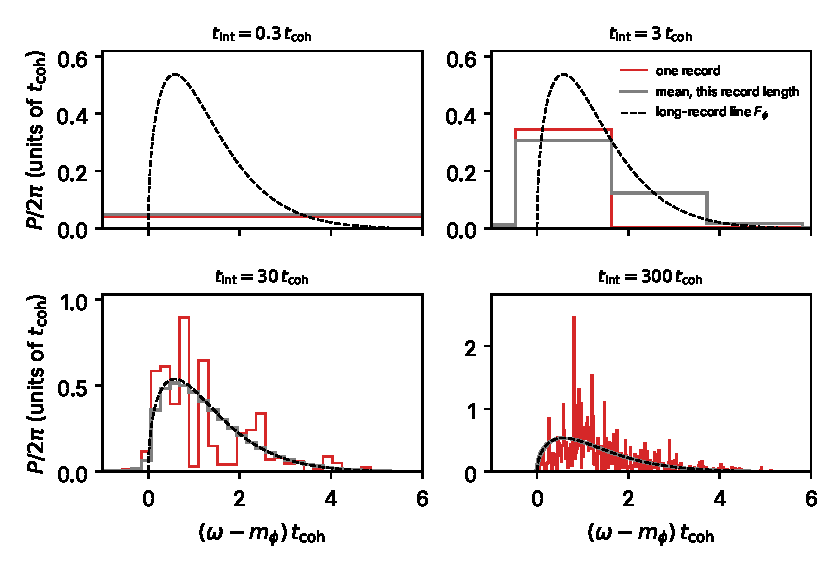
\includegraphics[width=0.92\linewidth]{figures/ch14/fig14_6.pdf}
  \caption{Periodogram of an axion-like field of unit mean power for records of $t_{\mathrm{int}} = 0.3$, 3, 30 and $300\,t_{\mathrm{coh}}$, against the energy above the rest energy in units of $1/t_{\mathrm{coh}} = m_\phi v_0^2$. Red: one Monte Carlo realization of the field, a sum of 3000 plane waves with random phases and with velocities from the standard halo of \cref{sec:1.2} seen from the Earth ($v_0 = \SI{238}{km/s}$, $v_{\mathrm{esc}} = \SI{544}{km/s}$, $v_E = \SI{250.5}{km/s}$). Bins of width $2\pi/t_{\mathrm{int}}$, one centered on the peak of the line. Gray: the mean periodogram for that record length, the line shape convolved with the Fejér kernel \cref{eq:14.6-fejer}. Dashed: the line shape $F_\phi$ of \cref{eq:14.6-Fphi}, the mean for a long record. Below $t_{\mathrm{coh}}$ one bin holds the whole line, with a height proportional to $t_{\mathrm{int}}$. Above it the bins resolve the line and scatter about it with the exponential distribution \cref{eq:14.6-expbin}.}
  \label{fig:14-spectrum}
\end{figure}

\begin{limitbox}[Gaussian-field signal and its power spectrum][lim:14.6b]
Exponential periodogram bins with mean $\mathsf{s}(\omega) \propto F_\phi(\omega)$, the line shape of \cref{eq:14.6-Fphi}, for a field built from Rayleigh-distributed amplitudes with random phases~\cite[Eqs.~(8), (10), (24)]{foster2018revealing}; for an absorber, the golden-rule mean of \cref{eq:8.2-abs} averaged over the line.
\par\smallskip
{\centering
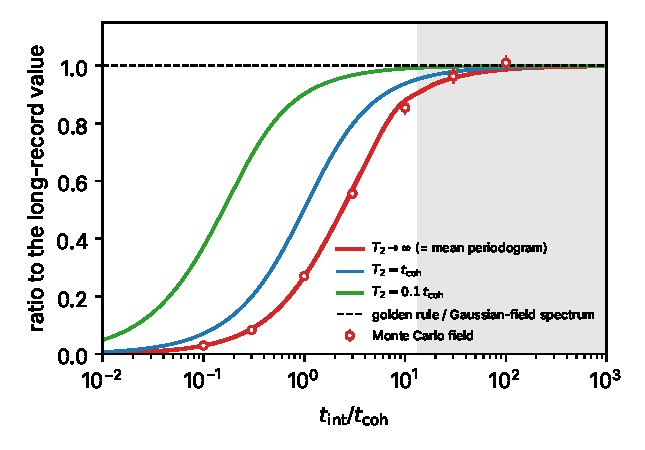
\includegraphics[width=0.92\linewidth]{figures/ch14/limit14_6b.pdf}
\captionof{figure}{Mean over the Gaussian field, for a record of length $t_{\mathrm{int}}$, divided by its long-record value, against $t_{\mathrm{int}}/t_{\mathrm{coh}}$. Red: the mean periodogram at the peak of the line, $\int\dd\omega\,F_\phi(\omega)\mathcal{K}_{t_{\mathrm{int}}}(\omega_{\mathrm{pk}} - \omega)/F_\phi(\omega_{\mathrm{pk}})$, which is also the energy absorbed by spins with $T_2 \to \infty$ at the peak frequency divided by the golden-rule value; circles: 1500 Monte Carlo realizations, with the scatter of their mean. Blue and green: energy absorbed by linearly driven spins with $T_2 = t_{\mathrm{coh}}$ and $0.1\,t_{\mathrm{coh}}$, divided by the golden-rule rate times $t_{\mathrm{int}}$. Standard halo of \cref{sec:1.2}. Gray band: the red curve within \SI{10}{\percent} of the long-record value, $t_{\mathrm{int}} \ge 13\,t_{\mathrm{coh}}$; for $T_2 = t_{\mathrm{coh}}$ and $0.1\,t_{\mathrm{coh}}$ the same accuracy needs $6.5\,t_{\mathrm{coh}}$ and $t_{\mathrm{coh}}$. The variance of the Monte Carlo bins equals the square of their mean within the sampling error, as the exponential law requires.}\label{fig:14-limit-spectrum}
\par}
\smallskip
Below $t_{\mathrm{coh}}$ and $T_2$ the mean grows as $t_{\mathrm{int}}^2$ rather than $t_{\mathrm{int}}$, with the ratio $t_{\mathrm{int}}/2\pi F_\phi(\omega_{\mathrm{pk}})$, and above them it approaches the golden rule as $1 - 1.25\,t_{\mathrm{coh}}/t_{\mathrm{int}}$, the leakage of the Fejér kernel.
\end{limitbox}

The bins of a stationary process are independent as long as the leakage of the Fejér kernel between neighbors is negligible. The likelihood of the periodogram is then the product of the distributions \cref{eq:14.6-expbin},
\begin{equation}
  -2\ln\mathsf{L} = 2\sum_k\Bigl[\ln\bar{\mathsf{P}}_k + \frac{\mathsf{P}_k}{\bar{\mathsf{P}}_k}\Bigr] ,
  \label{eq:14.6-like}
\end{equation}
the exponential-bin likelihood of Foster, Rodd and Safdi~\cite[Eq.~(29)]{foster2018revealing}, in which the signal enters through $\mathsf{s}_k$ and the coupling through its square, $\mathsf{s}_k \propto g^2$. Limits and discoveries follow from the likelihood ratio $\mathsf{t}$ of \cref{eq:C.14-ratio} and its thresholds \cref{eq:C.14-thresholds} (\cref{app:C.14}). How the sensitivity grows with $t_{\mathrm{int}}$ follows from the expected ratio for data without signal, $\mathsf{P}_k = \mathsf{b}_k$. Let $x_k = \mathsf{s}_k/\mathsf{b}_k$. Then $\mathsf{t} = 2\sum_k[\ln(1 + x_k) - x_k/(1 + x_k)]$, and for a weak signal, expanding to second order,
\begin{equation*}
  \mathsf{t} \simeq \sum_kx_k^2 = \frac{t_{\mathrm{int}}}{2\pi}\int\dd\omega\,\frac{\mathcal{S}_{\mathrm{sig}}(\omega)^2}{\mathcal{S}_{\mathrm{n}}(\omega)^2} ,
\end{equation*}
where the sum over bins of width $2\pi/t_{\mathrm{int}}$ became an integral. Let $\sigma_{\mathrm{sig}}^2$ be the mean square of the signal, proportional to $g^2$, and take white noise. For a record shorter than $t_{\mathrm{coh}}$ one bin holds the signal, $\mathsf{s} = \sigma_{\mathrm{sig}}^2t_{\mathrm{int}}$ and $\mathsf{b} = \mathcal{S}_{\mathrm{n}}$, so a fixed threshold on $\mathsf{t}$ means a fixed $x$, and
\begin{equation}
  \sigma_{\mathrm{sig}} \propto \mathcal{S}_{\mathrm{n}}^{1/2}\,t_{\mathrm{int}}^{-1/2}\quad(t_{\mathrm{int}} \ll t_{\mathrm{coh}}), \qquad
  \sigma_{\mathrm{sig}} \propto \mathcal{S}_{\mathrm{n}}^{1/2}\,(t_{\mathrm{int}}t_{\mathrm{coh}})^{-1/4}\quad(t_{\mathrm{int}} \gg t_{\mathrm{coh}}) .
  \label{eq:14.6-scaling}
\end{equation}
For a long record the integral gives $\mathsf{t} = 2\pi t_{\mathrm{int}}\sigma_{\mathrm{sig}}^4/(\Delta\omega_{\mathrm{eq}}\mathcal{S}_{\mathrm{n}}^2)$ with $\Delta\omega_{\mathrm{eq}} = 2.67/t_{\mathrm{coh}}$, which is the second law. Inside one coherence time the signal adds in amplitude and the noise in power, the familiar $t^{-1/2}$ of a coherent sinusoid. Beyond it the signal power stops growing in each bin, and only the number of bins over which the line is averaged grows, as $t_{\mathrm{int}}$, which halves the exponent. These are the scalings of Budker and collaborators~\cite[Eqs.~(A7), (A8)]{budker2014proposal}; the long-record form, with the coefficient of the weak-signal ratio, is the expected limit of Foster, Rodd and Safdi~\cite[Eqs.~(54), (63), (69)]{foster2018revealing}. For the spins, $\sigma_{\mathrm{sig}} = |M_\perp|$ is proportional to $g$, and the coupling at the threshold scales as $\sigma_{\mathrm{sig}}$.

The amplitude of the field within one coherence time is a random draw, and an analysis that ignores this sets too strong a limit. A search shorter than $t_{\mathrm{coh}}$ that takes the amplitude fixed at its mean value $\sqrt{2\rho_\chi}/m_\phi$ excludes every coupling whose signal would have exceeded the noise in that one realization; however, the field may have been weak during the record, with probability $1 - \ee^{-a}$ for an intensity below $a$ times its mean. Centers and collaborators found that limits with a fixed amplitude are too strong by a factor of 3 in a Bayesian treatment and 2.7 in a frequentist one, up to 10 with other priors, and 8.4 for gradient couplings~\cite[Eq.~(7)]{centers2021stochastic}. The exponential-bin likelihood already contains the random amplitude, so the correction is made once: with the likelihood \cref{eq:14.6-like}, or with a fixed-amplitude likelihood followed by the correction factor, never both.

An exact Neyman construction gives the size of the correction. Replace the line of the standard halo, convolved with the Fejér kernel, by $N_{\mathrm{eff}}$ equal bins, with $N_{\mathrm{eff}} = 1/\sum_kp_k^2$ the participation number of the bin fractions $p_k$ ($N_{\mathrm{eff}} \to 1$ below $t_{\mathrm{coh}}$ and $t_{\mathrm{int}}\Delta\omega_{\mathrm{eq}}/2\pi$ above). The bins have the width $2\pi/t_{\mathrm{int}}$, with one bin centered on the peak of the line. The statistic is the summed periodogram $\mathsf{Q}$ of those bins, with noise $\mathsf{b}$ per bin and total signal $\mathsf{s} = \sigma_{\mathrm{sig}}^2t_{\mathrm{int}}$ at every record length. With the Rayleigh amplitude of \cref{eq:14.6-expbin}, $\mathsf{Q}$ follows a Gamma distribution of shape $N_{\mathrm{eff}}$ and scale $\mathsf{b} + \mathsf{s}/N_{\mathrm{eff}}$; with a fixed amplitude and random phase, $2\mathsf{Q}/\mathsf{b}$ follows a noncentral $\chi^2$ distribution with $2N_{\mathrm{eff}}$ degrees of freedom and noncentrality $2\mathsf{s}/\mathsf{b}$. The \SI{95}{\percent} upper limit $\mathsf{s}_{\mathrm{up}}$ solves $P(\mathsf{Q} \le \mathsf{Q}_{\mathrm{obs}}\,|\,\mathsf{s}_{\mathrm{up}}) = 0.05$, with $\mathsf{Q}_{\mathrm{obs}}$ the median of the Gamma distribution of shape $N_{\mathrm{eff}}$ and scale $\mathsf{b}$ for data without signal. For the median of data without signal and one bin, $\mathsf{s}_{\mathrm{up}}/\mathsf{b} = 12.5$ with the Rayleigh amplitude and 3.17 with a fixed one, so that the fixed amplitude sets a coupling limit lower by $(12.5/3.17)^{1/2} = 1.99$. For data at the detection threshold, $\mathsf{Q}_{\mathrm{obs}} = \mathsf{b}\ln20$, the same construction gives 57.4 and 7.72 and a factor 2.73. \Cref{lim:14.6c} shows both treatments against the record length.
\begin{limitbox}[Sensitivity scalings of the exponential-bin likelihood][lim:14.6c]
Threshold amplitude $\propto\mathcal{S}_{\mathrm{n}}^{1/2}t_{\mathrm{int}}^{-1/2}$ for $t_{\mathrm{int}} < t_{\mathrm{coh}}$ and $\propto\mathcal{S}_{\mathrm{n}}^{1/2}(t_{\mathrm{int}}t_{\mathrm{coh}})^{-1/4}$ for $t_{\mathrm{int}} > t_{\mathrm{coh}}$~\cites[Eqs.~(A7), (A8)]{budker2014proposal}[Eqs.~(54), (63), (69)]{foster2018revealing}.
\par\smallskip
{\centering
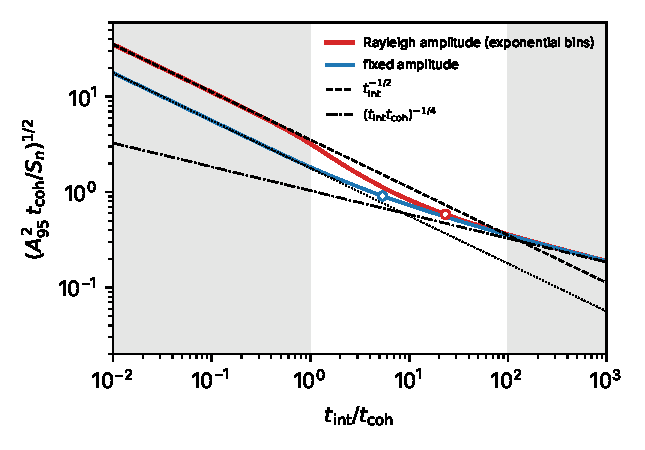
\includegraphics[width=0.92\linewidth]{figures/ch14/limit14_6c.pdf}
\captionof{figure}{Signal amplitude at the median expected \SI{95}{\percent} upper limit, $(\sigma_{\mathrm{sig}}^2t_{\mathrm{coh}}/\mathcal{S}_{\mathrm{n}})^{1/2}$, proportional to the coupling, against the record length over the coherence time, for white noise of spectrum $\mathcal{S}_{\mathrm{n}}$. Red: the signal as a Gaussian variable with a Rayleigh amplitude, the exponential-bin likelihood \cref{eq:14.6-like}. Blue: the signal power in each bin taken as fixed, with a random phase. Both curves follow from the Neyman construction of the text, with $N_{\mathrm{eff}}$ equal bins for the line of the standard halo of \cref{sec:1.2}. Dashed: $t_{\mathrm{int}}^{-1/2}$ for the Rayleigh amplitude (dotted: fixed amplitude); dash-dotted: $(t_{\mathrm{int}}t_{\mathrm{coh}})^{-1/4}$, common to both. Circles: the crossover, where the local slope is $-3/8$, at $23\,t_{\mathrm{coh}}$ (Rayleigh) and $5.4\,t_{\mathrm{coh}}$ (fixed). Gray: the Rayleigh curve within \SI{10}{\percent} of the $t_{\mathrm{int}}^{-1/2}$ law ($t_{\mathrm{int}} \le t_{\mathrm{coh}}$) or of the $(t_{\mathrm{int}}t_{\mathrm{coh}})^{-1/4}$ law ($t_{\mathrm{int}} \ge 100\,t_{\mathrm{coh}}$).}\label{fig:14-limit-scaling}
\par}
\smallskip
Neither power law holds between $t_{\mathrm{coh}}$ and $100\,t_{\mathrm{coh}}$, where the Rayleigh curve falls as steeply as $t_{\mathrm{int}}^{-0.67}$, faster than either law, because the record begins to average over independent amplitudes.
\end{limitbox}

The fixed amplitude sets a limit lower by 1.99 for records below $t_{\mathrm{coh}}$, by 1.76 at $t_{\mathrm{coh}}$ and by \SI{1.5}{\percent} at $100\,t_{\mathrm{coh}}$. The two power laws, extended, meet at $136\,t_{\mathrm{coh}}$ for the Rayleigh amplitude and at $8.7\,t_{\mathrm{coh}}$ for the fixed one, so the crossover lies between a few and about a hundred coherence times and its coefficient is not universal.

\begin{workedexample}{The scaling crossover for a \SI{1}{neV} axion-like field}\label{we:14-crossover}
An axion-like field of $m_\phi = \SI{1}{neV}$ oscillates at $m_\phi/2\pi = \SI{241.8}{kHz}$. By \cref{eq:14.6-tcoh}, $t_{\mathrm{coh}} = \SI{1.044}{s}$, and its line has the equivalent width $\Delta\omega_{\mathrm{eq}}/2\pi = 2.67/(2\pi t_{\mathrm{coh}}) = \SI{0.41}{Hz}$, $1.7\times10^{-6}$ of the frequency.

A $^{207}$Pb sample resonates at this frequency in $B_0 = 241.8\,\mathrm{kHz}/(9.034\,\mathrm{MHz\,T^{-1}}) = \SI{26.8}{mT}$. Its $T_2 = \SI{16.7}{ms}$ is $0.016\,t_{\mathrm{coh}}$, so the spin line, of half width $1/T_2 = \SI{60}{s^{-1}}$, is 63 times wider than the field line, $m_\phi v_0^2 = \SI{0.96}{s^{-1}}$. The spins are in the case $T_2 \ll t_{\mathrm{coh}}$ of \cref{lim:14.6a}: the magnetization reaches the steady state of \cref{eq:14.6-mperp} after a few $T_2$, about \SI{0.05}{s}, and its amplitude then follows the Rayleigh amplitude of the field, which changes on the scale of a second.

The sensitivity depends on how long a record at one frequency can be. With the construction of \cref{lim:14.6c}, the threshold coupling falls by a factor 3.46 from $t_{\mathrm{int}} = \SI{0.1}{s}$ to \SI{1}{s}, more than the $\sqrt{10} = 3.16$ of the coherent law, since the record starts to sample a second amplitude. The local slope reaches $-3/8$ at $23\,t_{\mathrm{coh}} = \SI{24}{s}$. A record of one hour spans 3447 coherence times and a day 82\,730. Going from an hour to a day improves the limit by 2.24, close to $24^{1/4} = 2.21$ and far from the $24^{1/2} = 4.9$ that a coherent signal would give. At \SI{0.1}{s} the fixed-amplitude analysis would claim a limit 1.99 times lower; at one hour the two agree to better than \SI{0.1}{\percent}.
\end{workedexample}

A search that scans the field over a decade of frequency in a fixed total time spends less time at each frequency as the line narrows toward low masses. The crossover then decides whether to dwell longer at one frequency or to scan more. At $m_\phi = \SI{1}{\micro eV}$, $t_{\mathrm{coh}} = \SI{1.04}{ms}$, and every practical record lies deep in the $(t_{\mathrm{int}}t_{\mathrm{coh}})^{-1/4}$ regime; at \SI{1}{peV}, $t_{\mathrm{coh}} = \SI{17}{min}$, and the random amplitude must be in the likelihood.
